\section{Типичная схема эволюционного алгоритма.}
\begin{itemize}
     Нужно решить задачу оптимизации. На каждом этапе особи проходят отбор (выживание). Если особи не улучшают показатели, то  нет смысла впускать их в новую популяцию.  \\
     \\
Упрощенная эволюция, выполняемая на компьютере:\\
- Особи: решения некоторой задачи оптимизации \\
- Приспособленность: насколько хорошо данное решение\\
- Мутация: внесение небольших изменений в решение\\
- Скрещивание: построение решения из фрагментов двух и более решений\\
\\
Схема представлена на рисунке 1
\end{itemize}
\begin{figure}[h]
\centering
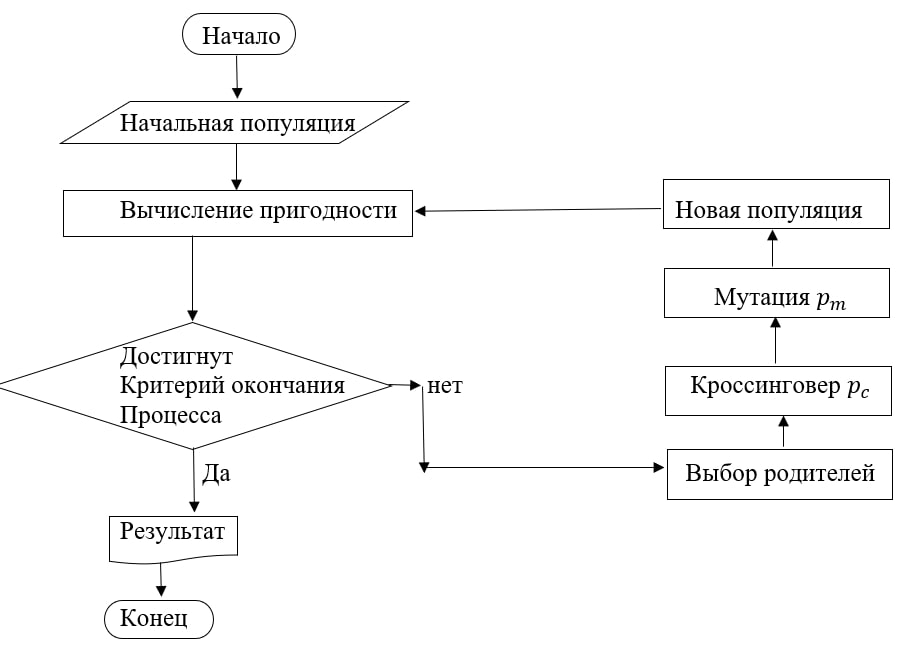
\includegraphics[width=0.8\linewidth]{images/Sxema.jpg}
\caption{Схема генетического алгоритма}
\label{fig:mpr}
\end{figure}
